\documentclass{elsarticle}
\usepackage{hyperref}
\usepackage[utf8]{inputenc}
\usepackage{wrapfig}
\usepackage{amsmath}
\usepackage{amsthm}
\usepackage{amssymb}
\usepackage[tmargin=1in,bmargin=1in]{geometry}
\usepackage{caption}
\usepackage{graphicx}
\usepackage{latexsym}
\usepackage{pdfsync}
\usepackage[boxed]{algorithm}
\usepackage{algorithm}
%\usepackage{algpseudocode}
\usepackage{multirow}
\usepackage{rotating}
\usepackage{color}
\usepackage{url}
\usepackage{subfigure}
\usepackage{bigstrut}
\usepackage{bigints}
\usepackage[normalem]{ulem}

\usepackage[normalem]{ulem}




\hypersetup{
    colorlinks=true,              % false: boxed links; true: colored links
    linkcolor=blue,               % color of internal links
    citecolor=blue,               % color of links to bibliography
    filecolor=black,              % color of file links
    urlcolor=red,               % color of external links
    bookmarks=false,
    pdffitwindow=true,
    pdfpagelayout=SinglePage
}

\captionsetup[figure]{font=small,labelfont=normal}

\definecolor{mypink}{cmyk}{0, 0.7808, 0.4429, 0.1412}

\definecolor{mybrown}{cmyk}{0, 0.60, 0.95, 0.63}
\definecolor{darkgreen}{cmyk}{0.98, 0, 0.36, 0.22}


\newcommand{\comment}[1]{\textcolor{red}{[#1]$_{\rm Frederic}$}}
\newcommand{\pouriacomment}[1]{\textcolor{darkgreen}{[#1]$_{\rm Pouria}$}}

\newcommand{\etal}{\textit{et al.\ }}
\newcommand{\pd}[2]{\frac{\partial #1}{\partial #2}}
\newcommand{\mbf}[1]{\mathbf{#1}}
\newcommand{\vect}[1]{\boldsymbol{#1}}
\newcommand{\tensor}[1]{\underline{\underline{\boldsymbol{#1}}}}
\newcommand{\mat}[1]{\underline{\underline{\boldsymbol{#1}}}}
\newcommand{\be}{\begin{equation}}
\newcommand{\ee}{\end{equation}}
\newcommand{\ben}{\begin{equation*}}
\newcommand{\een}{\end{equation*}}
\newcommand{\bea}{\begin{eqnarray}}
\newcommand{\eea}{\end{eqnarray}}
\newcommand{\bean}{\begin{eqnarray*}}
\newcommand{\eean}{\end{eqnarray*}}

\newcommand{\fphi}[2]{\frac{\phi_#1}{\phi_#1-\phi_#2}}
\newcommand{\lif}[2]{\frac{f_#1\phi_#2-f_#2\phi_#1}{\phi_#2-\phi_#1}}
\newcommand{\dx}{{\Delta x}}
\newcommand{\dy}{{\Delta y}}
\newcommand{\dz}{{\Delta z}}
\newcommand{\dt}{{\Delta t}}
\newcommand{\hf}{{\frac12}}
\newcommand{\U}{\vect{U}}
\newcommand{\n}{\vect{n}}



\usepackage{algorithm}
\usepackage[noend]{algpseudocode}
\makeatletter
\def\BState{\State\hskip-\ALG@thistlm}
\makeatother



\begin{document}
\title{JAX-DIPS: Differentiable Interfacial PDE Solver}

\cortext[cor]{Corresponding author: p.a.mistani@gmail.com}


\author[1]{Pouria A. Mistani\thanks{corresponding author} $^{\dagger,}$}
\author[2]{Samira Pakravan$^{\dagger,}$}
\author[1]{Rajesh Ilango}
\author[2]{Frederic G. Gibou}

\address[1]{NVIDIA Corporation, Santa Clara, CA 95051, USA}
\address[2]{University of California, Santa Barbara, CA 93106-5070, USA}

\begin{abstract}
	We present an end-to-end differentiable PDE solver supporting both forward and inverse free boundary problems using the level-set method. We implemented this framework using JAX, extending support for CPU/GPU/TPU platforms. Algorithmically, our proposed framework builds on the blended inverse PDE solver architecure (BiPDE) that authors have proposed earlier \cite{pakravan2021solving}. JAX-DIPS is an open-source software package published is available at \href{https://github.com/JAX-DIPS/JAX-DIPS}{https://github.com/JAX-DIPS/JAX-DIPS}.

\end{abstract}

\begin{keyword}
	level-set method \sep free boundary problems \sep inverse problems \sep jump conditions \sep differentiable programming
\end{keyword}

\maketitle
\def\thefootnote{$\dagger$}\footnotetext{These authors contributed equally to this work}







%%%%%%%%%%%%%%%%%%%%%%%%%%%%%%%%%%%%%
%%%%%%%%%%%%%%%%%%%%%%%%%%%%%%%%%%%%%
\section{Introduction}
\label{sec::introduction}
Differentiable programming ...

DTO vs OTD: we are doing DTO which is Discretize then Optimize paradigm. OTD is the traditional adjoint methods.

JAX-DIPS Poisson problem solver provides the two sides of $A u =b$ which is obtained after discretization of the governing PDE problem over a uniform 3D grid. Two solution schemes for the forwards problem are possible: (1) using usual iterative methods having left-hand-side and right-hand-side of the PDE discretization, and (2) using autodifferentiation across loss function (difference between lhs and rhs in 2-norm) with respect to a given estimate for the solution vector on the underlying grid $\rm u_{ijk}$. Both approaches focus on minimizing the residual over the grid points
\begin{align*}
	\min_{u_{ijk}} \vert\vert Au -b \vert \vert^2_2
\end{align*}
The first method attempts to span the residual space in an iterative fashion by \textit{estimating} the gradient of the minimizing function, while the second method offered in JAX-DIPS is directly computing the exact gradient of the minimizing function with respect to the current estimate for solution. Therefore, the advantage of this method is fewer iterations and faster convergence specially for irregular geometries where the condition number of the linear system leads to much difficulties that need to be resolved by complex preconditioning and increased number of iterations.



\section{Numerical Scheme for Free Boundary Problems}
Consider a closed irregular interface ($\rm \Gamma$) that partitions the computational domain ($\rm \Omega$) into interior ($\rm \Omega^-$) and exterior ($\rm \Omega^+$) subdomains; \textit{i.e.}, $\rm \Omega=\Omega^- \cup \Gamma \cup \Omega^+$. We are interested in the solutions $\rm u^\pm\in \Omega^\pm$ to the following class of linear elliptic problems in  $\rm \mathbf{x}\in\Omega^\pm$:
\begin{align*}
	 & k^{\pm}u^{\pm} - \nabla \cdot (\mu^{\pm}\nabla u^\pm)=f^{\pm}, & \mathbf{x}\in\Omega^\pm \\
	 & [u]=\alpha,                                                    & \mathbf{x} \in \Gamma   \\
	 & [\mu \partial_{\mathbf{n}}u]=\beta,                            & \mathbf{x} \in \Gamma
\end{align*}
Here $f^\pm=f(\mathbf{x} \in \Omega^\pm)$ is the spatially varying source term, $\rm \mu^\pm=\mu(\mathbf{x} \in \Omega^\pm)$  are the diffusion coefficients, and $k^\pm$ are the reaction coefficients in the two domains. We consider Dirichlet boundary conditions in a cubic domain $\rm \Omega=[-L/2,L/2]^3$.



\subsection{Interpolation methods}
To support finite discretization methods for the free boundary problems (namely solver, level-set method, and geometric integrations) a widely needed building block is the ability to interpolate field values anywhere inside a grid cell given the values on the grid points. In \texttt{JAX-DIPS} we currently implement two types of interpolation schemes that have been used in the context of the level set method for achieving second-order accurate solutions by Min \& Gibou (2007a)\cite{MIN2007300}: (i) trilinear interpolation, and (ii) quadratic non-oscillatory interpolation.


\subsubsection{Trilinear interpolation}
In a unit grid cell, rescaled to $\mathcal{C}\in [0,1]^3$, the trilinear interpolation at a point $(x,y,z)\in \mathcal{C}$ uses the grid values on the parent cell vertices according to equation 11 of \cite{MIN2007300},
\begin{align*}
 \phi(x,y,z)= \sum_{i,j,k\in {0,1}} \phi(i,j,k) (-1)^{i+j+k}(1-x-i)(1-y-j)(1-z-k)
\end{align*}
Trilinear interpolation is based on polynomials of order 1 and offers accuracy of order 2 using 8 immediate vertices in a grid cell.

\subsubsection{Quadratic non-oscillatory interpolation}
Quadratic interpolation extends the trilinear interpolation by adding second order derivatives of the interpolating field. This is needed because trilinear interpolation is sensitive to presence of discontinuities and kinks which are abundant in the context of free boundary problems. The extension reads
\begin{align*}
	\phi(x,y,z)= &\sum_{i,j,k\in {0,1}} \phi(i,j,k) (-1)^{i+j+k}(1-x-i)(1-y-j)(1-z-k) \\
				& - \phi_{xx} \frac{x(1-x)}{2} - \phi_{yy} \frac{y(1-y)}{2}- \phi_{zz} \frac{z(1-z)}{2} 
\end{align*}
where second order derviatives are sampled as the minimum value on the parent cell vertices to enhance numerical stability of the interpolation
\begin{align*}
	\phi_{xx} & = \min_{v \in \textrm{vertices}(\mathcal{C})} \vert D_{xx} \phi_v \vert \\
	\phi_{yy} & = \min_{v \in \textrm{vertices}(\mathcal{C})} \vert D_{yy} \phi_v \vert \\
	\phi_{zz} & = \min_{v \in \textrm{vertices}(\mathcal{C})} \vert D_{zz} \phi_v \vert
\end{align*}
The second order derivative operator is the familiar 5-point finite difference stencil.




\subsection{Level-set method}
The level-set method for solving free boundary problems was introduced by Osher \& Sethian (1988) \cite{osher1988fronts}. The free boundary is described as the zero contour of a signed-distance function, $\phi$, whose evolution is given by the advection equation according to some velocity field dictated by the physics of the problem, $\mathbf{v}$, that is defined over the moving boundary
\begin{align}
	\frac{\partial \phi}{\partial t} + \mathbf{v}\cdot \nabla \phi = 0
\end{align}

This \textit{implicit} representation of the moving boundaries resolves the need for the challenging task of adapting the underlying grid to the yet-unknown discontinuities in the solution field. The computational simplicity of using Cartesian grids for solving free boundary problems with irregular geometries, as well as the ability to simulate freely moving discontinuities in a \textit{sharp}-manner, that is required by the physics of these problems, are the two main offerings of the level-set method for this class of PDE problems.

The signed-distance property of the level-set function, \textit{i.e.} $\vert \nabla \phi\vert =1 $, deteriorates with timestepping the discretized advection equation. This is resolved by solving the Sussman reinitialization equation \cite{SUSSMAN1994146} in fictitious time ($\tau$) every few iterations of the physical time ($t$),
\begin{align}
	\frac{\partial \phi}{\partial \tau} + sgn(\phi_0) (\vert \nabla \phi \vert - 1) = 0 \label{eq::sussman}
\end{align}

Note the asymptotic solution of the Sussman equation is the signed-distance property of the level-set function. Here $sgn(\phi_0)$ is the sign function evaluated on the level-set function before reinitialization in order to preserve the sign of grid points during the fictitous updates.

Besides implicit representation of the free boundaries, the level-set function can be used to compute normal vectors to the interface 
\begin{align*}
	\mathbf{n} = \nabla\phi / \vert \nabla \phi \vert 
\end{align*}
as well as the curvature of the interface
\begin{align*}
	\kappa = \nabla \cdot \mathbf{n}
\end{align*}



Below we describe numerical methods implementd in \texttt{JAX-DIPS} to solve the level-set equations.

\subsubsection{Second order accurate semi-Lagrangian advection scheme}
Semi-Lagrangian methods are unconditionally stable for solving advection equations, therefore avoiding the restrictive CFL condition on the timestep size from time $t^n$ to $t^{n+1}$. The general procedure to solve for $\phi^{n+1}(\mathbf{x}^{n+1})$ is to first evaluate for each grid point, $\mathbf{x}^{n+1}$, the departure point, $\mathbf{x}_d$, in the upwind direction along the characteristic curve; then use interpolation methods to recover value of the solution field at the departure point; and finally updating the solution field by setting $\phi^{n+1}(\mathbf{x}^{n+1})=\phi^n(\mathbf{x}_d)$.

The task of evaluating departure points is treated by the second-order mid-point method \cite{XIU2001658}
\begin{align*}
	\hat{\mathbf{x}} &= \mathbf{x}^{n+1} - \frac{\Delta t}{2} \cdot \mathbf{v}^n(\mathbf{x}^{n+1})\\
	\mathbf{x}_d &= \mathbf{x}^{n+1} - \Delta t \cdot \mathbf{v}^{n+\frac{1}{2}}(\hat{\mathbf{x}})
\end{align*}

The first step is trivial, but the second step demands velocity at the mid-timestep $t^{n + \frac{1}{2}}$ which can be evaluated from the velocity field at the previous two timesteps, $t^n$ and $t^{n-1}$, according to
\begin{align*}
	\mathbf{v}^{n+\frac{1}{2}} = \frac{3}{2}\mathbf{v}^n - \frac{1}{2} \mathbf{v}^{n-1}
\end{align*}
this intermediate velocity field is then fed into a trilinear interpolation scheme to sample the velocities on the intermediate points $\mathbf{v}^{n+\frac{1}{2}}(\hat{\mathbf{x}})$. At this point departure points can be computed, and the advected solution is updated by sampling a nonoscillatory interpolant of the level-set function at timestep $t^n$ over the computed departure points $\phi^n(\mathbf{x}_d)$.


\subsubsection{Godunov Hamiltonian for reinitialization}
The Sussman equation \ref{eq::sussman} is generically discretized over its spatial dimensions to obtain
\begin{align}
	\frac{d\phi}{d\tau} = -sgn(\phi^0) \bigg[ H_G(D_x^+\phi, D_x^-\phi, D_y^+\phi, D_y^-\phi, D_z^+\phi, D_z^-\phi, ) - 1 \bigg]
\end{align}
where $H_G$ is the so-called Gudonov Hamiltonian defined as
\begin{align*}
	H_G(a,b,c,d,e,f) &= \sqrt{ \sum_{(i,j)\in (a,b),(c,d),(e,f)}\max\bigg( \vert\min( s\cdot i,0)\vert^2, \vert\max( s\cdot j,0)\vert^2 \bigg)  }\\
	s&= sgn(\phi^0)
\end{align*}
where the one-sided derivatives are computed using second order accurate discretizations in the bulk far from interfaces
\begin{align*}
	&(D_x^+\phi)_{i,j,k} = \frac{\phi_{i+1,j,k} - \phi_{i,j,k}}{\Delta x} - \frac{\Delta x}{2} \textrm{minmod}((D_{xx}\phi)_{i,j,k}, (D_{xx}\phi)_{i+1,j,k})\\
	&(D_x^-\phi)_{i,j,k} = \frac{\phi_{i,j,k} - \phi_{i-1,j,k}}{\Delta x} + \frac{\Delta x}{2} \textrm{minmod}((D_{xx}\phi)_{i,j,k}, (D_{xx}\phi)_{i-1,j,k})
\end{align*}
where we used $\textrm{minmod}(a,b)\triangleq \textrm{median}(a,0,b)$ slope-limiter \cite{shu1988efficient}; and in the vicinity of interfaces these derivatives take into account distance to the interface using the level-set function. With similar results along $y$ and $z$ axes, the derivative along the positive $x$-axis is given by 
\begin{align*}
 &(D_x^+\phi)_{i,j,k} = \frac{0 - \phi_{i,j,k}}{s_I} - \frac{s_I}{2} c_2^+\\
 & s_I = \frac{\Delta x}{2} + \left\{
 \begin{array}{ll}
 	-c_0^+/c_1^+    & \textrm{if} \ \vert c_2^+\vert<\epsilon \\
 	\bigg(-c_1^+ - sgn(\phi^0_{i,j,k})\sqrt{(c_1^+)^2 - 4c_2^+ c_0^+} \bigg)/(2 c_2^+)    & \textrm{if} \ \vert c_2^+\vert\ge \epsilon 
 \end{array}
\right.
\end{align*}
where 
\begin{align*}
	c_2^+ &= \textrm{minmod}((D_{xx}\phi)_{i,j,k}, (D_{xx}\phi)_{i+1,j,k}) \\
	c_1^+ &=  \frac{\phi_{i+1,j,k} - \phi_{i,j,k}}{\Delta x} \\
	c_0^+ &= \frac{\phi_{i+1,j,k} + \phi_{i,j,k}}{2} - \frac{c_2^+ (\Delta x)^2}{4}
\end{align*}
And along the negative $x$-axis we obtain
\begin{align*}
 &(D_x^-\phi)_{i,j,k} = \frac{\phi_{i,j,k} - 0}{s_I} + \frac{s_I}{2} c_2^-\\
 & s_I = \frac{\Delta x}{2} + \left\{
 \begin{array}{ll}
 	c_0^-/c_1^-    & \textrm{if} \ \vert c_2^-\vert<\epsilon \\
 	\bigg(c_1^- - sgn(\phi^0_{i,j,k})\sqrt{(c_1^-)^2 - 4c_2^- c_0^-} \bigg)/(2 c_2^-)    & \textrm{if} \ \vert c_2^-\vert\ge \epsilon 
 \end{array}
\right.
\end{align*}
where 
\begin{align*}
	c_2^- &= \textrm{minmod}((D_{xx}\phi)_{i,j,k}, (D_{xx}\phi)_{i-1,j,k}) \\
	c_1^- &= \frac{\phi_{i,j,k} - \phi_{i-1,j,k}}{\Delta x} \\
	c_0^- &= \frac{\phi_{i-1,j,k} + \phi_{i,j,k}}{2} - \frac{c_2^- (\Delta x)^2}{4}
\end{align*}


Having the right-hand-side, the TVD-RK2 method of Shu \& Osher \cite{shu1988efficient} is applied to the update the level-set function in fictitious time
\begin{align*}
	\tilde{\phi}^{n+1}&=\phi^n - \Delta \tau \cdot sgn(\phi^0) [ H_G^n -1] \\
	\tilde{\phi}^{n+2}&=\tilde{\phi}^{n+1} - \Delta \tau \cdot sgn(\phi^0) [ \tilde{H}_G^{n+1} -1] \\
	\phi^{n+1}&=\frac{\phi^n + \tilde{\phi}^{n+2}}{2}
\end{align*}
with a timestep chosen by $\Delta \tau = \min (s_I, \Delta x, \Delta y, \Delta z) / 3$.

\subsection{Integration over 3D surfaces and volumes}
We use uniform Cartesian grids. For computational cells that are crossed by the interface, \textit{i.e.} $\mathcal{V}_{i,j,k}\cap \Gamma \neq 0$, we use the geometric integrations proposed by Min \& Gibou (2007b) \cite{min2007geometric}. In this scheme each grid cell, $\mathcal{C}$, is decomposed into five tetrahedra by the middle-cut triangulation \cite{sallee1984middle} (each cell is rescaled to $[0,1]^3$) that are described below (also see figure 1 (right) of \cite{min2007geometric}):
\begin{align*}
	 & \rm S_1 \equiv conv(P_{000} ; P_{100} ; P_{010} ; P_{001}) & \rm{ x = 0\ face,\ y = 0\ face,\ z = 0\ face} \\
	 & \rm S_2 \equiv conv(P_{110} ; P_{100} ; P_{010} ; P_{111}) & \rm{ x = 1\ face,\ y = 1\ face,\ z = 0\ face} \\
	 & \rm S_3 \equiv conv(P_{101} ; P_{100} ; P_{111} ; P_{001}) & \rm{ x = 1\ face,\ y = 0\ face,\ z = 1\ face} \\
	 & \rm S_4 \equiv conv(P_{011} ; P_{111} ; P_{010} ; P_{001}) & \rm{ x = 0\ face,\ y = 1\ face,\ z = 1\ face} \\
	 & \rm S_5\equiv conv(P_{111} ; P_{100} ; P_{010} ; P_{001})  & \rm{ no\ face\ exposure}
\end{align*}

Hence each 3D grid cell is the union of $5$ tetrahedra (simplices) $\mathcal{C}=\cup_{i=1}^5 S_i$, where each simplex is identified by the pre-existing vertices of the grid cell (hence not creating new grid points). Given the values of the level set function sampled at these vertices one can compute coordinates of intersection points of the interface with each of the simplices $S_i \cap \Gamma $ as well as the negative domain $S_i \cap \Omega^-$. If ${P_0,\cdots, P_3}$ are the four vertices of a simplex $S$, then $\Gamma$ crosses an edge $P_i P_j$ if and only if $\phi(P_i)\phi(P_j)<0$ and the intersection point across this edge is given by linear interpolation:
\begin{align*}
P_{ij}=P_j \frac{\phi(P_i)}{\phi(P_i) - \phi(P_j)} - P_i \frac{\phi(P_j)}{\phi(P_i) - \phi(P_j)}
\end{align*}

Number of negative level-set values on the $4$ (in 3D) tetrahedron vertices classifies the specific configuration for intersection between simplex $S$ and the interface through a variable $\eta(\phi, S)=n({P_i | \phi(P_i)<0})$. In 3D, possible values are $\eta =0,1,2,3,4$ that correspond to the four configurations for the intersection cross section enumerated below:
\begin{itemize}
\item $S\cap\Gamma$, see table 2 and figure 2 of \cite{min2007geometric}:
	\begin{itemize}
		\item $\eta=0$: tetrahedron ($S$) is completely in positive domain with no intersection, $S\cap\Gamma=\emptyset$.
		\item $\eta=1$: with a single vertex in negative domain and remaining three in positive domain, the tetrahedron and interface have exactly $3$ intersection points, the simplex $S\cap\Gamma$ has exactly $3$ vertices; \textit{cf.}, see figure 2 (center) of  \cite{min2007geometric}.   
		\item $\eta=2$: with two vertices in negative domain and remaining two in positive domain, the cross section has four vertices that is splitted into two 3-vertex simplices; \textit{cf.}, see figure 2 (right) of  \cite{min2007geometric}.
		\item $\eta=3$: with one vertex in positive domain and remaining three vertices in negative domain, the cross section has 3 vertices that is computed by inverting the sign of the level-set values on vertices and following the instruction for case $\eta=1$.
		\item $\eta=4$: tetrahedron is completely in negative domain with no intersection, $S\cap\Gamma=\emptyset$.
	\end{itemize}

\item $S\cap \Omega^-$, see table 4 and figure 4 of \cite{min2007geometric}:
	\begin{itemize}
		\item $\eta=0$: tetrahedron is completely in positive domain with no intersection, $S\cap\Omega^-=\emptyset$; 
		\item $\eta=1$: the intersection $S\cap\Omega^-$ is characterized by a single tetrahedron with 4 vertices according to figure 4 (left) of \cite{min2007geometric}; \textit{i.e.}, one vertex is the negative level-set vertex of the parent tetrahedron and three others are interpolated points over the three edges pertaining to the negative vertex.
		\item $\eta=2$: the intersection $S\cap\Omega^-$ is characterized by three tetrahedra with 12 vertices according to figure 4 (center) of \cite{min2007geometric}. Note that there 
		\item $\eta=3$: the intersection $S\cap\Omega^-$ is characterized by three tetrahedra with 12 vertices according to figure 4 (right) of \cite{min2007geometric}.
		\item $\eta=4$: tetrahedron is completely in negative domain and $S\cap\Omega^-=S$; 
	\end{itemize}

\end{itemize}


Note that although we only need to allocate memory for at most 4 vertices to uniquely identify $S\cap\Gamma$, in \texttt{JAX-DIPS} we choose to pre-allocate memory for two 3-vertex simplex data structure per $S$ with a total of $6$ vertices to separately store information for the cross section geometry. Similarly for $S\cap \Omega^-$ we pre-allocate memory for a three 4-vertex simplex data structure per $S$. Altogether, in the current implementation the geometric information of intersection points for each simplex $S$ is expressed in terms of 5 simplicies (2 three-vertex simplices for surface area and 3 four-vertex simplicies for volume) using 18 points; this is an area for future optimization.




Having the intersection points, we compute surface and volume integrals of a given field over the interface $\Gamma$ and in negative domain $\Omega^-$ as a summation of integrals over the identified simplices. For each simplex (with $n=3$ or $n=4$ vertices) surface and volume integrals can be numerically computed by having these vertices ${P_0,\cdots, P_n}$ and the values of the field $f$ at these vertices according to 
\begin{align*}
\int_S f dx = \textrm{vol}(S)\cdot \frac{f(P_0) + \cdots + f(P_n)}{n+1}
\end{align*}
where
\begin{align*}
\textrm{vol}(S) = \frac{1}{n!} \bigg\vert \textrm{det} \begin{pmatrix}
(P_1-P_0)\hat{e}_1 & \cdots & (P_n-P_0)\hat{e}_1 \\
\vdots  & \ddots & \vdots  \\
(P_1-P_0)\hat{e}_n  & \cdots & (P_n-P_0)\hat{e}_n 
\end{pmatrix} \bigg\vert
\end{align*}
with $\hat{e}_i$ being the $i^{th}$ Cartesian unit basis vector.





\subsection{Cross sections of interface with grid cell faces}
For the numerical discretizations considered in this work we also need the surface areas for simplices created at the intersection of $\Gamma$ with each of the 6 faces of a grid cell $\mathcal{C}$. In \texttt{JAX-DIPS} for each face we reuse two corresponding simplices exposed to that face that were calculated in the geometric integrations module, explicitly: 
\begin{itemize}
	\item $x=0$ face has contributions from ($S_1$, $S_4$)
	\item $x=1$ face has contributions from ($S_2$, $S_3$)
	\item $y=0$ face has contributions from ($S_1$, $S_3$)
	\item $y=1$ face has contributions from ($S_2$, $S_4$)
	\item $z=0$ face has contributions from ($S_1$, $S_2$)
	\item $z=1$ face has contributions from ($S_3$, $S_4$)
\end{itemize}
For each face, we extract vertices from $(S_i,S_j)$-pair that lie on the considered face and sum the surface areas in (negative domain) contributed from each simplex on that face; therefore, the portion of the face surface area in the positive domain is simply the complementing value $\rm area^+=area_{face}-area^-$; \textit{i.e.}, this ensures sum of areas adds up to the exact face area in downstream computations.







\subsection{Finite discretization method}\label{sec::FD}

For spatial discretizations at the presence of jump conditions we employ the numerical algorithm proposed by Bochkov and Gibou (2020) \cite{bochkov2020solving} (BG20) on Cartesian grids. BG20 produces second-order accurate solutions and first-order accuracte gradients in the $L^\infty$-norm, while having a compact stencil that makes it a good candidate for parallelization. Moreover, treatment of the interface jump conditions do not introduce any augmented variables, this preserves the homogeneous structure of the linear system.

Here we use a finite volume discretization equation uniformly for all grid points. At grid points where the finite volumes are crossed by $\rm \Gamma$ we have

\begin{align*}
	 & \sum_{s=-,+}\int_{\Omega^s \cap \mathcal{V}_{i,j}}  k^{s} u^{s} d\Omega -\sum_{s=-,+} \int_{\Omega^s\cap \partial\mathcal{V}_{i,j}} \mu^{s}\partial_{\mathbf{n}^s} u^s  d\Gamma = \sum_{s=-,+}\int_{\Omega^s \cap \mathcal{V}_{i,j}}  f^{s} d\Omega + \int_{\Gamma \cap \mathcal{V}_{i,j}}[\mu\partial_{\mathbf{n}}u]d\Gamma \\
	\intertext{following standard treatment of volumetric integrals and using central differencing for derivatives we obtain in 2D (with trivial 3D extension)}
	 & \sum_{s=-,+} k_{i,j}^s u_{i,j}^{s} |\mathcal{V}_{i,j}^s| - \sum_{s=-,+}\bigg( \mu_{i-\frac{1}{2},j}^s A_{i-\frac{1}{2},j}^s\frac{u_{i-1,j}^s - u_{i,j}^s}{\Delta x}     +   \mu_{i+\frac{1}{2},j}^s A_{i+\frac{1}{2},j}^s\frac{u_{i+1,j}^s - u_{i,j}^s}{\Delta x} +                                                          \\
	 & \mu_{i, j-\frac{1}{2}}^s A_{i, j-\frac{1}{2}}^s\frac{u_{i,j-1}^s - u_{i,j}^s}{\Delta y} + \mu_{i, j+\frac{1}{2}}^s A_{i, j+\frac{1}{2}}^s\frac{u_{i,j+1}^s - u_{i,j}^s}{\Delta y} \bigg)                                                                                                                                     \\
	 & =  \sum_{s=-,+} f_{i,j}^{s} |\mathcal{V}_{i,j}^s| + \int_{\Gamma\cap \mathcal{V}_{i,j}} \beta d\Gamma + \mathcal{O}(\max(\Delta x, \Delta y)^\mathcal{D})
\end{align*}
where $\mathcal{D}$ is the problem dimensionality.

\begin{figure}
	\centering
	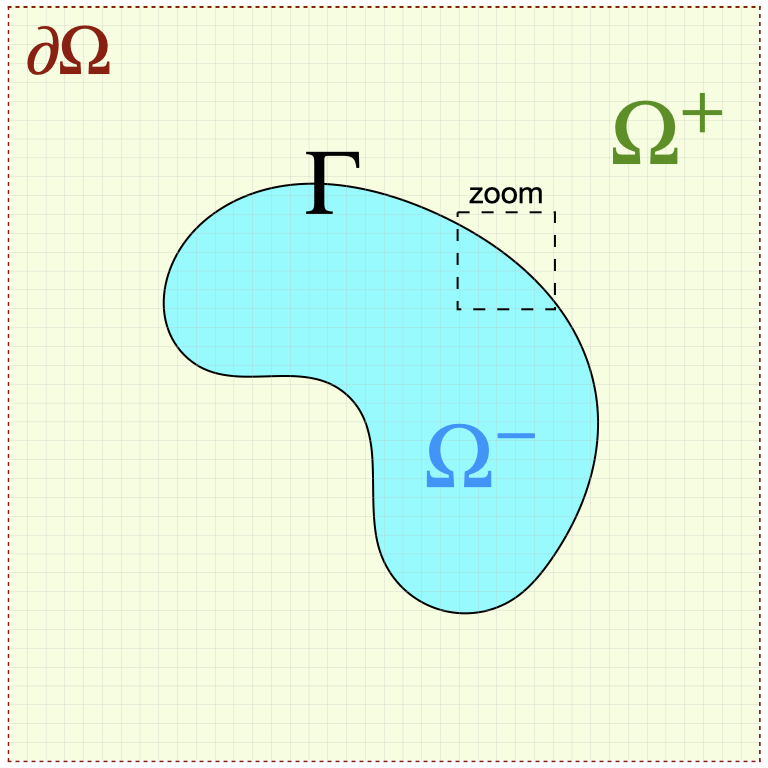
\includegraphics[width=0.45\linewidth]{./figures/grids_full.png}
	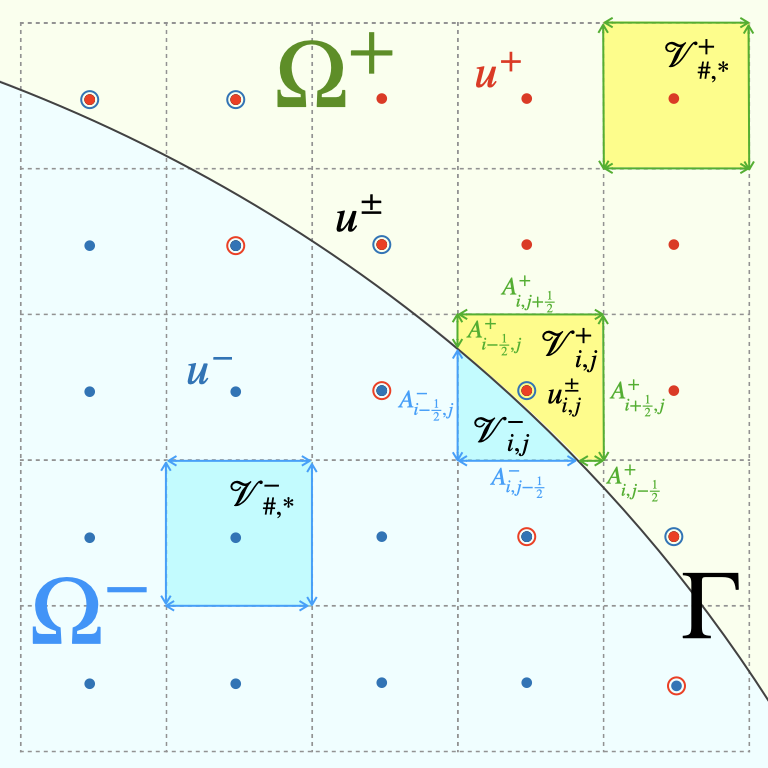
\includegraphics[width=0.45\linewidth]{./figures/grids.png}
	\caption{Notation used in this paper. Close to the interface where finite volumes are crossed by the interface, there are extra degrees of freedom (open circles) that are extrapolations of solutions from each domain to the opposite domain. Jump conditions are implicitly encoded in these extrapolated values.}
	\label{fig:grid}
\end{figure}

Note that far from interface either $s=-$ (for $\mathbf{x}\in \Omega^-$) or $s=+$ (for $\mathbf{x}\in \Omega^+$) is retained. This is automatically considered through zero values for sub-volumes $|\mathcal{V}_{i,j}^+|$ and $|\mathcal{V}_{i,j}^-|$ as well as their face areas. Note that $\mu_{i-1/2,j}^-$ (or $\mu_{i-1/2,j}^+$) corresponds to the value of diffusion coefficient at the middle of segment $A^-_{i-1/2,j}$ (or $A^+_{i-1/2,j}$) respectively, same is true for other edges as well. However, there are extra degrees of freedom on grid points whose finite volumes are crossed by the interface; \textit{i.e.}, see double circles in figure \ref{fig:grid}. Bochkov and Gibou derived analytical expressions for the extra degrees of freedom ($u^+$ in $\Omega^-$ and $u^-$ in $\Omega^+$) in terms of the original degrees of freedom ($u^-$ in $\Omega^-$ and $u^+$ in $\Omega^+$) as well as the jump conditions, this preserves the original $\rm N_x \times N_y$ system size.

In this scheme the basic idea is to extrapolate the jump at grid point from jump condition at the projected point onto the interface using a Taylor expansion: $u^+_{i,j} - u^-_{i,j}=[u]_{\mathbf{r}_{i,j}^{pr}} + \delta_{i,j}(\partial_\mathbf{n}u^+(\mathbf{r}^{pr}_{i,j}) - \partial_\mathbf{n}u^-(\mathbf{r}^{pr}_{i,j})) $. The unknown value ($u^-_{i,j}$ or $u^+_{i,j}$) is obtained based on approximation of the normal derivatives (\textit{i.e.} $\partial_\mathbf{n}u^\pm(\mathbf{r}^{pr}_{i,j})$) which are computed using a least squares calculation on neighboring grid points that are in the fast-diffusion region (referred to as ``Bias Fast'') or in the slow diffusion region (referred to as ``Bias Slow''). This makes two sets of ruls for unknown values $u^\pm_{i,j}$.

In two dimensions and on uniform grids, the gradient operator at the grid cell $(i,j)$ that is crossed by an interface is estimated by a least squares solution given by
\begin{align*}
	 & (\nabla u^\pm)_{i,j} = \mathbf{D}^\pm_{i,j} \begin{bmatrix}
		u_{i-1,j-1} - u^\pm_{i,j} \\
		u_{i,j-1} - u^\pm_{i,j}   \\
		\vdots                    \\
		u_{i+1,j+1} - u^\pm_{i,j}
	\end{bmatrix} & \mathbf{D}^\pm_{i,j} = \big(X^T_{i,j} W^\pm_{i,j} X_{i,j} \big)^{-1} \big( W^\pm_{i,j} X_{i,j} \big)^T
\end{align*}
and
\begin{align*}
	 & W^\pm_{i,j} = \begin{bmatrix}
		 & \omega^\pm_{i,j} (-1,-1) &                         &        &                        \\
		 &                          & \omega^\pm_{i,j} (0,-1) &        &                        \\
		 &                          &                         & \ddots &                        \\
		 &                          &                         &        & \omega^\pm_{i,j} (1,1) \\
	\end{bmatrix} & X_{i,j} = \begin{bmatrix}
		 & -h_x & -h_y \\
		 & 0    & -h_y \\
		 & h_x  & -h_y \\
		 & -h_x & 0    \\
		 & 0    & 0    \\
		 & h_x  & 0    \\
		 & -h_x & h_y  \\
		 & 0    & h_y  \\
		 & h_x  & h_y
	\end{bmatrix}
\end{align*}
and
\begin{equation}
	\omega_{i,j}^\pm (p,q) = \begin{cases}
		1 & (p,q)\in N_{i,j}^\pm \\
		0 & \text{else}
	\end{cases}
\end{equation}
In this case, $D^\pm_{i,j}$ is a $2\times 9$ matrix and we denote each of its $2\times 1$ columns with $d^\pm_{i,j,p,q}$
\begin{align*}
	\mathbf{D}^\pm_{i,j}  = \begin{bmatrix}
		 & d^\pm_{i,j,-1,-1} & d^\pm_{i,j,0,-1} & d^\pm_{i,j,1,-1} & d^\pm_{i,j,-1,0} & d^\pm_{i,j,0,0} & d^\pm_{i,j,1,0} & d^\pm_{i,j,-1,1} & d^\pm_{i,j,0,1} & d^\pm_{i,j,1,1}
	\end{bmatrix}
\end{align*}
The least square coefficients are then obtained by dot product of normal vector with these columns
\begin{align*}
	c^\pm_{i,j,p,q} = \mathbf{n}_{i,j}^T  d^\pm_{i,j,p,q}
\end{align*}
and normal derivative can be computed (noting that $c_{i,j}^\pm =-\sum_{(p,q)\in N_{i,j}^\pm}c_{i,j,p,q}^\pm$)
\begin{align*}
\partial_n u^\pm (\mathbf{r}^{proj}_{i,j})= c_{i,j}^\pm u_{i,j}^\pm + \sum_{(p,q)\in N_{i,j}^\pm} c_{i,j,p,q}^\pm u_{i+p, j+q}^\pm + \mathcal{O}(h) 
\end{align*}

At this point we can define a few intermediate variables at each grid point to simplify the presentation of the method,
\begin{align*}
	 & \zeta_{i,j,p,q}^\pm := \delta_{i,j} \frac{[\mu]}{\mu^\mp}c_{i,j,p,q}^\pm  & \zeta_{i,j}^\pm := -\sum_{(p,q)\in N_{i,j}^\pm} \zeta_{i,j,p,q}^\pm   \\
	 & \gamma_{i,j,p,q}^\pm := \frac{\zeta_{i,j,p,q}^\pm}{1 \pm \zeta^\pm_{i,j}} & \gamma^\pm_{i,j} := -\sum_{(p,q)\in N_{i,j}^\pm} \gamma_{i,j,p,q}^\pm
\end{align*}
where the set of neighboring grid points are
\begin{align*}
	N_{i,j}^\pm = \{(p,q) :\ \ \  p=-1,0,1, \ \ \  q=-1,0,1, \ \ \ (p,q)\neq (0,0), \ \ \ \mathbf{x}_{i+p,j+q}\in \Omega^\pm \}
\end{align*}
and $\delta_{i,j}$ is the signed distance from $\mathbf{x}_{i,j}$ that is computed from the level-set function $\phi(\mathbf{x})$
\begin{align*}
	\delta_{i,j}=\frac{\phi(\mathbf{x}_{i,j})}{|\nabla \phi(\mathbf{x}_{i,j})|}
\end{align*}

\begin{itemize}
	\item Rules based on approximating $\partial_\mathbf{n}u^+(\mathbf{r}^{pr}_{i,j})$:
\end{itemize}
%\begin{equation}
% u_{i,j}^-=\begin{cases}
%    u_{i,j}, & \text{ $\mathbf{x}_{i,j}\in \Omega^-$}\\
%    u_{i,j} - \alpha_1 -\delta_{i,j}\frac{\beta_1}{\mu^{+}} - \delta_{i,j} \frac{[\mu]}{\mu^+} \bigg( \frac{ c_{i,j}^- (u_{i,j} - \alpha_1 - \delta_{i,j}\frac{\beta_1}{\mu^+}) + \sum_{(p,q)\in N_{i,j}^-} c_{i,j,p,q}^- u_{i+p,j+q}  }{ 1 - \delta_{i,j}\frac{[\mu]}{\mu^+}c_{i,j}^- }\bigg), & \text{ $\mathbf{x}_{i,j}\in \Omega^+$}
%  \end{cases}
%\end{equation}
%\begin{equation}
% u_{i,j}^+=\begin{cases}
%    u_{i,j} + \alpha_1 + \delta_{i,j}\frac{\beta_1}{\mu^{+}} - \delta_{i,j} \frac{[\mu]}{\mu^+}\big( c_{i,j}^- u_{i,j}  + \sum_{(p,q)\in N_{i,j}^-} c_{i,j,p,q}^- u_{i+p,j+q} \big), & \text{ $\mathbf{x}_{i,j}\in \Omega^-$}\\
%    u_{i,j}, & \text{ $\mathbf{x}_{i,j}\in \Omega^+$}
%  \end{cases}
%\end{equation}

\begin{equation}
	u_{i,j}^-=\begin{cases}
		u_{i,j}                                                                                                                                                 & \text{ $\mathbf{x}_{i,j}\in \Omega^-$} \\
		u_{i,j} (1 - \gamma_{i,j}^- ) - \sum_{(p,q)\in N_{i,j}^-} \gamma_{i,j,p,q}^- u_{i+p,j+q} - (\alpha + \frac{\delta_{i,j}\beta}{\mu^+})(1-\gamma^-_{i,j}) & \text{ $\mathbf{x}_{i,j}\in \Omega^+$}
	\end{cases}
\end{equation}
\begin{equation}
	u_{i,j}^+=\begin{cases}
		u_{i,j}(1 - \zeta^-_{i,j} ) - \sum_{(p,q)\in N_{i,j}^-} \zeta^-_{i,j,p,q}u_{i+p,j+q}  + \alpha + \delta_{i,j}\frac{\beta}{\mu^+} & \text{ $\mathbf{x}_{i,j}\in \Omega^-$} \\
		u_{i,j}                                                                                                                          & \text{ $\mathbf{x}_{i,j}\in \Omega^+$}
	\end{cases}
\end{equation}
It is useful to cast this in the form of matrix operations through defining intermediate tensors:
\begin{align*}
	 & \boldsymbol{\Gamma}_{i,j} := \begin{bmatrix}
		 & \gamma_{i-1,j+1}^- & \gamma^-_{i,j+1} & \gamma^-_{i+1,j+1} \\
		 & \gamma_{i-1,j}^-   & \gamma^-_{i,j}   & \gamma^-_{i+1,j}   \\
		 & \gamma_{i-1,j-1}^- & \gamma^-_{i,j-1} & \gamma^-_{i+1,j-1}
	\end{bmatrix}, & \boldsymbol{\zeta}_{i,j} := \begin{bmatrix}
		 & \zeta^-_{i-1,j+1} & \zeta^-_{i,j+1} & \zeta^-_{i+1,j+1} \\
		 & \zeta^-_{i-1,j}   & \zeta^-_{i,j}   & \zeta^-_{i+1,j}   \\
		 & \zeta^-_{i-1,j-1} & \zeta^-_{i,j-1} & \zeta^-_{i+1,j-1}
	\end{bmatrix} \\
	 & \mathbf{U}_{i,j} := \begin{bmatrix}
		 & u_{i-1,j+1} & u_{i,j+1} & u_{i+1, j+1} \\
		 & u_{i-1,j}   & u_{i,j}   & u_{i+1, j}   \\
		 & u_{i-1,j-1} & u_{i,j-1} & u_{i+1, j-1}
	\end{bmatrix},          & \mathbf{N}^\pm_{i,j} :=\begin{bmatrix}
		 & \omega_{i,j}^\pm(-1,1)  & \omega_{i,j}^\pm(0,1)  & \omega_{i,j}^\pm(1,1)  \\
		 & \omega_{i,j}^\pm(-1,0)  & 0                      & \omega_{i,j}^\pm(1,0)  \\
		 & \omega_{i,j}^\pm(-1,-1) & \omega_{i,j}^\pm(0,-1) & \omega_{i,j}^\pm(1,-1) \\
	\end{bmatrix}
\end{align*}
where $\mathbf{N^-}$ is a masking filter that passes the values in the negative neighborhood of node $(i,j)$.

We also introduce the Hadamard product $\odot$ between two identical matrices that creates another identical matrix with each entry being elementwise products. Moreover, double contraction of two tensors $A$ and $B$ is defined by $A : B = \sum A \odot B$ which is a scalar value and equals the sum of all entries of the Hadamard product of the tensors; \textit{i.e.}, note $A:A$ is square of Frobenius norm of $A$. Using these notations, the substitution rules read
\begin{equation}
	u_{i,j}^-=\begin{cases}
		u_{i,j}                                                                                                                                                                                                                                                                        & \text{ $\mathbf{x}_{i,j}\in \Omega^-$} \\
		\big(1 + \boldsymbol{\Gamma}^-_{i,j} : \mathbf{N}^-_{i,j}  \big) u_{i,j} -  \big( \boldsymbol{\Gamma}^-_{i,j}  \odot \mathbf{N}^-_{i,j} \big) : \mathbf{U}_{i,j}  - (\alpha + \delta_{i,j}\frac{\beta}{\mu^+}) \big(1 + \boldsymbol{\Gamma}^-_{i,j} : \mathbf{N}^-_{i,j} \big) & \text{ $\mathbf{x}_{i,j}\in \Omega^+$}
	\end{cases}
\end{equation}
\begin{equation}
	u_{i,j}^+=\begin{cases}
		\big(1 + \boldsymbol{\zeta}^-_{i,j} : \mathbf{N}^-_{i,j}   \big) u_{i,j} - \big( \boldsymbol{\zeta}^-_{i,j}  \odot \mathbf{N}^-_{i,j}  \big) : \mathbf{U}_{i,j} + \alpha + \delta_{i,j}\frac{\beta}{\mu^+} & \text{ $\mathbf{x}_{i,j}\in \Omega^-$} \\
		u_{i,j}                                                                                                                                                                                                    & \text{ $\mathbf{x}_{i,j}\in \Omega^+$}
	\end{cases}
\end{equation}



\begin{itemize}
	\item Rules based on approximating $\partial_\mathbf{n}u^-(\mathbf{r}^{pr}_{i,j})$:
\end{itemize}
%\begin{equation}
% u_{i,j}^-=\begin{cases}
%    u_{i,j}, & \text{ $\mathbf{x}_{i,j}\in \Omega^-$}\\
%    u_{i,j} - \alpha_1 -\delta_{i,j}\frac{\beta_1}{\mu^{-}} - \delta_{i,j} \frac{[\mu]}{\mu^-} \big( c_{i,j}^+ u_{i,j} + \sum_{(p,q)\in N_{i,j}^+} c_{i,j,p,q}^+ u_{i+p,j+q} \big) , & \text{ $\mathbf{x}_{i,j}\in \Omega^+$}
%  \end{cases}
%\end{equation}
%\begin{equation}
% u_{i,j}^+=\begin{cases}
%    u_{i,j} + \alpha_1 + \delta_{i,j}\frac{\beta_1}{\mu^{-}} - \delta_{i,j} \frac{[\mu]}{\mu^-} \bigg( \frac{ c_{i,j}^+ (u_{i,j} + \alpha_1 + \delta_{i,j}\frac{\beta_1}{\mu^-}) + \sum_{(p,q)\in N_{i,j}^+} c_{i,j,p,q}^+ u_{i+p,j+q}  }{ 1 + \delta_{i,j}\frac{[\mu]}{\mu^-}c_{i,j}^+ }\bigg), & \text{ $\mathbf{x}_{i,j}\in \Omega^-$} \\
%    u_{i,j}, & \text{ $\mathbf{x}_{i,j}\in \Omega^+$}\\
%  \end{cases}
%\end{equation}
\begin{equation}
	u_{i,j}^-=\begin{cases}
		u_{i,j}                                                                                                                        & \text{ $\mathbf{x}_{i,j}\in \Omega^-$} \\
		u_{i,j} (1-\zeta^+_{i,j}) - \sum_{(p,q)\in N_{i,j}^+} \zeta_{i,j,p,q}^+ u_{i+p,j+q} - \alpha - \delta_{i,j}\frac{\beta}{\mu^-} & \text{ $\mathbf{x}_{i,j}\in \Omega^+$}
	\end{cases}
\end{equation}
\begin{equation}
	u_{i,j}^+=\begin{cases}
		u_{i,j}(1 - \gamma^+_{i,j}) - \sum_{(p,q)\in N^+_{i,j}} \gamma^+_{i,j,p,q} u_{i+p, j+q} + (\alpha + \delta_{i,j}\frac{\beta}{\mu^-})(1 - \gamma^+_{i,j}) & \text{ $\mathbf{x}_{i,j}\in \Omega^-$} \\
		u_{i,j}                                                                                                                                                  & \text{ $\mathbf{x}_{i,j}\in \Omega^+$} \\
	\end{cases}
\end{equation}
in matrix notation we have
\begin{equation}
	u_{i,j}^-=\begin{cases}
		u_{i,j}                                                                                                                                                                                                 & \text{ $\mathbf{x}_{i,j}\in \Omega^-$} \\
		\big(1 + \boldsymbol{\zeta}^+_{i,j} : \mathbf{N}^+_{i,j}\big) u_{i,j}  -  \big( \boldsymbol{\zeta}^+_{i,j} \odot \mathbf{N}^+_{i,j} \big) : \mathbf{U}_{i,j} - \alpha - \delta_{i,j}\frac{\beta}{\mu^-} & \text{ $\mathbf{x}_{i,j}\in \Omega^+$}
	\end{cases}
\end{equation}
\begin{equation}
	u_{i,j}^+=\begin{cases}
		\big(1 + \boldsymbol{\Gamma}^+_{i,j} : \mathbf{N}^+_{i,j}\big) u_{i,j} - \big( \boldsymbol{ \Gamma}^+_{i,j} \odot  \mathbf{N}^+_{i,j}  \big) : \mathbf{U}_{i,j} + (\alpha + \delta_{i,j}\frac{\beta}{\mu^-})\big(1 + \boldsymbol{\Gamma}^+_{i,j} : \mathbf{N}^+_{i,j} \big) & \text{ $\mathbf{x}_{i,j}\in \Omega^-$} \\
		u_{i,j}                                                                                                                                                                                                                                                                     & \text{ $\mathbf{x}_{i,j}\in \Omega^+$} \\
	\end{cases}
\end{equation}



\begin{algorithm}
	\caption{Bias Slow approximation of the non-existing solution value on a grid point based on existing solution values in its neighborhood. The notation is used for $u_{i,j}^\pm=B_{i,j}^\pm : \mathbf{U}_{i,j}+r_{i,j}^\pm$.}\label{euclid}
	\begin{algorithmic}[1]
		\Procedure{Bias Slow}{}
		\If {$\Gamma \cap \mathcal{C}_{i,j}= \emptyset$}
		\State $B_{i,j}^\pm=\begin{bmatrix}
				0 & 0 & 0 \\
				0 & 1 & 0 \\
				0 & 0 & 0 \\
			\end{bmatrix};\ \ r^\pm_{i,j}=0$
		\Else
		\If {$\mu_{i,j}^- > \mu_{i,j}^+$}
		\If {$\phi_{i,j}\ge 0$}
		\State $B_{i,j}^+=\begin{bmatrix}
				0 & 0 & 0 \\
				0 & 1 & 0 \\
				0 & 0 & 0 \\
			\end{bmatrix};\ \ r^+_{i,j}=0$
		\State $B_{i,j}^-=\begin{bmatrix}
				-\gamma_{i,j,-1,1}^-  & -\gamma_{i,j,0,1}^-  & -\gamma_{i,j,1,1}^-  \\
				-\gamma_{i,j,-1,0}^-  & 1-\gamma^-_{i,j}     & -\gamma_{i,j,1,0}^-  \\
				-\gamma_{i,j,-1,-1}^- & -\gamma_{i,j,0,-1}^- & -\gamma_{i,j,1,-1}^- \\
			\end{bmatrix};\ \ r^-_{i,j}=-(\alpha_{i,j}^{proj} + \delta_{i,j}\frac{ \beta_{i,j}^{proj}}{\mu_{proj}^+}) (1 - \gamma_{i,j}^-)$
		\Else

		\State $B_{i,j}^+=\begin{bmatrix}
				-\zeta_{i,j,-1,1}^-  & -\zeta_{i,j,0,1}^-  & -\zeta_{i,j,1,1}^-  \\
				-\zeta_{i,j,-1,0}^-  & 1-\zeta^-_{i,j}     & -\zeta_{i,j,1,0}^-  \\
				-\zeta_{i,j,-1,-1}^- & -\zeta_{i,j,0,-1}^- & -\zeta_{i,j,1,-1}^- \\
			\end{bmatrix};\ \ r^+_{i,j}=\alpha_{i,j}^{proj} + \delta_{i,j}\frac{ \beta_{i,j}^{proj}}{\mu_{proj}^+}$

		\State $B_{i,j}^-=\begin{bmatrix}
				0 & 0 & 0 \\
				0 & 1 & 0 \\
				0 & 0 & 0 \\
			\end{bmatrix};\ \ r^-_{i,j}=0$

		\EndIf

		\Else




		\If {$\phi_{i,j}\ge 0$}
		\State $B_{i,j}^+=\begin{bmatrix}
				0 & 0 & 0 \\
				0 & 1 & 0 \\
				0 & 0 & 0 \\
			\end{bmatrix};\ \ r^+_{i,j}=0$
		\State $B_{i,j}^-=\begin{bmatrix}
				-\zeta_{i,j,-1,1}^+  & -\zeta_{i,j,0,1}^+  & -\zeta_{i,j,1,1}^+  \\
				-\zeta_{i,j,-1,0}^+  & 1-\zeta^+_{i,j}     & -\zeta_{i,j,1,0}^+  \\
				-\zeta_{i,j,-1,-1}^+ & -\zeta_{i,j,0,-1}^+ & -\zeta_{i,j,1,-1}^+ \\
			\end{bmatrix};\ \ r^-_{i,j}=\alpha_{i,j}^{proj} + \delta_{i,j}\frac{ \beta_{i,j}^{proj}}{\mu_{proj}^-}$
		\Else

		\State  $B_{i,j}^+=\begin{bmatrix}
				-\gamma_{i,j,-1,1}^+  & -\gamma_{i,j,0,1}^+  & -\gamma_{i,j,1,1}^+  \\
				-\gamma_{i,j,-1,0}^+  & 1-\gamma^+_{i,j}     & -\gamma_{i,j,1,0}^+  \\
				-\gamma_{i,j,-1,-1}^+ & -\gamma_{i,j,0,-1}^+ & -\gamma_{i,j,1,-1}^+ \\
			\end{bmatrix};\ \ r^+_{i,j}=(\alpha_{i,j}^{proj} + \delta_{i,j}\frac{ \beta_{i,j}^{proj}}{\mu_{proj}^-}) (1 - \gamma_{i,j}^+)$

		\State $B_{i,j}^-=\begin{bmatrix}
				0 & 0 & 0 \\
				0 & 1 & 0 \\
				0 & 0 & 0 \\
			\end{bmatrix};\ \ r^-_{i,j}=0$

		\EndIf


		\EndIf

		\EndIf

		%\BState \emph{top}:
		%\If {$i > \textit{stringlen}$} \Return false
		%\EndIf
		%\State $j \gets \textit{patlen}$
		%\BState \emph{loop}:
		%\If {$\textit{string}(i) = \textit{path}(j)$}
		%\State $j \gets j-1$.
		%\State $i \gets i-1$.
		%\State \textbf{goto} \emph{loop}.
		%\State \textbf{close};
		%\EndIf
		%\State $i \gets i+\max(\textit{delta}_1(\textit{string}(i)),\textit{delta}_2(j))$.
		%\State \textbf{goto} \emph{top}.
		\EndProcedure
	\end{algorithmic}
\end{algorithm}





\subsection{Neural network approximators for the solution}

In 1987, Hecht and Nielson \cite{hecht1987kolmogorov} applied an improved version of Kolmogorov's 1957 superposition theorem \cite{kolmogorov1957representation}, due to Sprecher \cite{sprecher1965structure}, to the field of neurocomputing and demonstrated that a $3$-layer feedforward neural network (one input layer with $n$ inputs, one hidden layer with $2n+1$ neurons, one output layer) are universal approximators for all \textit{continuous} functions from the $n$-dimensional cube to a finite $m$-dimensional real vector space; \textit{i.e.}, $f: [0,1]^n \rightarrow \mathbb{R}^m $. Recently, Ismailov (2022) \cite{ismailov2022} demonstrated existence of neural networks implementing \textit{discontinuous} functions, however efficient learning algorithms for such networks are not still available. 

The solutions of interfacial PDE problems are discontinuous, with jumps appearing not only in the solution but also in the solution gradient. In light of above considerations, we define two separate neural networks to represent solution in $\Omega^-$ and $\Omega^+$ regions:
\begin{align*}
& u^+ = \mathcal{N}^+(\mathbf{x}): \mathbb{R}^3\cap \Omega^+ \rightarrow \mathbb{R}  & u^- = \mathcal{N}^-(\mathbf{x}): \mathbb{R}^3\cap \Omega^- \rightarrow \mathbb{R}
\end{align*}

In each network we implement two hidden layers with $10$ neurons per layer using \texttt{tanh} activation function and the output layer is a single linear neuron. Note that piecewise differentiable nonlinearities such as the \texttt{ReLU} function are inappropriate choices for representing solutions to differential equations. Weights and biases are initialized from a truncated normal distribution with zero mean and unit variance. There are a total of $322$ trainable parameters.

Solution networks are evaluated on grid points while the parameters of these networks are optimized using the loss function.



\subsection{Differentiable solution strategy}

We define the loss function by the 2-norm of the residual of the discretized partial differential equation with jump conditions derived in section \ref{sec::FD} that is evaluated on the grid points:
\begin{align*}
	&\mathcal{L}(u) = \vert\vert A\hat{u}(\mathbf{x}_{ijk}\in \Omega) - b\vert\vert_2^2 + \textrm{vol}_{\mathcal{C}}\vert\vert \hat{u}(\mathbf{x}_{ijk}\in\partial \Omega) - u(\mathbf{x}_{ijk}\in\partial \Omega)\vert\vert_2^2 
\end{align*}
JAX-DIPS allows for exact computation of the gradient of the loss function using automatic differentiation, \textit{i.e.} $\nabla_u \mathcal{L}(u)$. This is advantageous over existing approximate iterative methods (with preconditioning) such as GMRES, Conjugate Gradient, \textit{etc}. Therefore, our strategy is to leverage this capability and use more sophisticated optimizers developed in the deep learning community (\textit{e.g.} Adam \cite{kingma2014adam}, RMSProp, \textit{etc}) to minimize the afforementioned loss function with the desired solution vector $\rm u^\ast$ of the PDE problem.

Solving an interfacial PDE problem on a $\rm 128\times 128 \times 128$ grid is therefore equivalent to a deep neural network architecture with $2,097,152$ trainable parameters. Besides number of trainable parameters, the computational complexity of the algebraic operations in solving a PDE system with provided discretizations closely resembles computational complexity of convolutional operations with kernel sizes equivalent to the stencil size of the discretization method (in this case $3\times 3 \times 3$).


First order methods are slow but cheap; second order methods are fast but expensive. In \texttt{JAX-DIPS} we primarily utilize first order optimization methods such as Adam, RMSProp, etc. Second order methods such as Newton or BFGS are certainly faster convergence but require much more memory. Traditionally used GMRES or Conjugate Gradient methods for sparse linear systems are somewhere between first order and second order optimization methods that are based on build a basis vectors by computing gradients that are conjugate to each other $\mathbf{p}_j^T A \mathbf{p}_i=0$ and will converge to the solution in at most $n$ steps; \textit{i.e.}, at most the solution vector is spanned in the full basis.


\subsubsection{Gradient based optimization with learning rate annealing}

We found that starting from a zero guess for the solution it is important to start from a large learning rate and gradually decay the learning rate in a process of exponential annealing. For this purpose, we use the exponential decay scheduler provided by \texttt{Optax} \cite{optax2020github} to control the learning rate in the Adam \cite{kingma2014adam} optimizer:
\begin{align*}
r_{k} = r_0 \alpha^{k / T}
\end{align*}
where $r_k$ is the learning rate at step $k$ of optimization, $\alpha<1$ is the decay rate, and $T$ is the decay count-scale. By default, we set $T=100$, $\alpha=0.975$, starting from an initial value of $r_0=10^{-2}$ and clip gradients by maximum global gradient norm (to a value $1$) \cite{gradClipping} before applying the Adam updates in each step. We note a larger decay rate, \textit{e.g.} $\alpha=0.98$, leads to small oscillations after $10000$ steps and although similar levels of accuracy can be achieved at much less iterations, here we report results with the more robust decay rate. See figure \ref{fig::optimization} for an example of loss evolution during optimization.

\begin{figure}[ht]
\centering
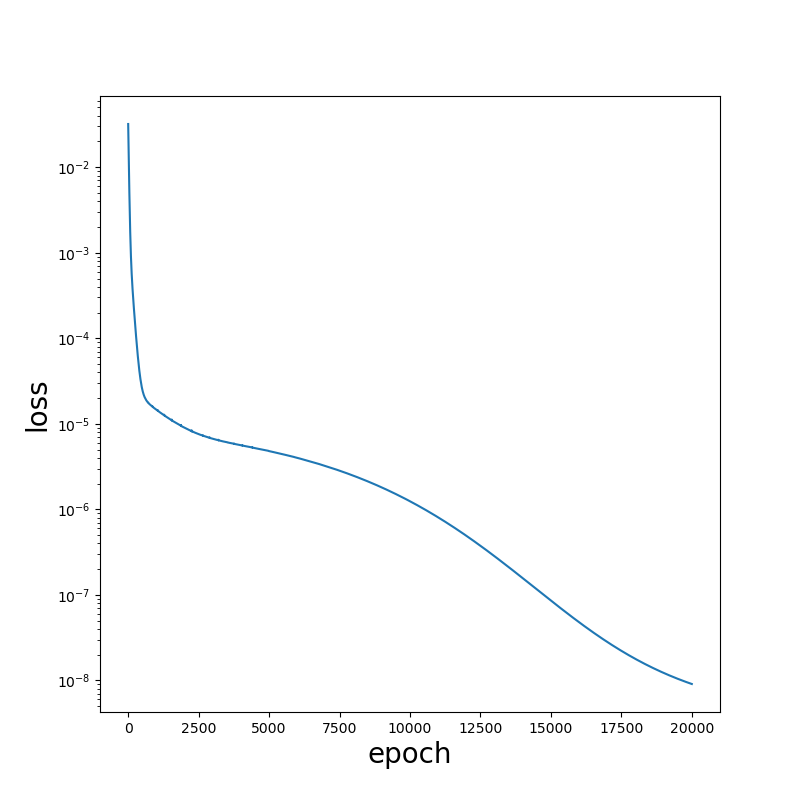
\includegraphics[width=0.85\linewidth]{figures/poisson_solver_loss_with_annealing.png}
\caption{Effect of annealing to dampen learning rate with number of epochs. }
\label{fig::optimization}
\end{figure}








\section{Numerical Examples}

\begin{align*}
	 & k^{\pm}u^{\pm} - \nabla \cdot (\mu^{\pm}\nabla u^\pm)=f^{\pm}, & \mathbf{x}\in\Omega^\pm \\
	 & [u]=\alpha,                                                    & \mathbf{x} \in \Gamma   \\
	 & [\mu \partial_{\mathbf{n}}u]=\beta,                            & \mathbf{x} \in \Gamma
\end{align*}



We present successively more complex test cases and analyze performance of \texttt{JAX-DIPS} in each case.


\subsection{No interface, $\Gamma=\emptyset $}
We set the level-set function to $\phi(\mathbf{x})=\sqrt{x^2 + y^2 + z^2} + 0.5$ within a domain $\Omega:[-1,1]^3$ characterizing absence of all jump conditions. Using the method of manufactured solutions, we construct the following Poisson problem for an exact solution $u(\mathbf{x}) = \sin(y)\cos(x)$ with appropriate Dirichlet boundary conditions:
\begin{align*}
	 - \Delta u &=2\sin(y)\cos(x), & \mathbf{x}\in\Omega\\
	 u(\mathbf{x}) &= \sin(y)\cos(x), &\mathbf{x}\in \partial \Omega
\end{align*}
with \texttt{Adam} optimizer starting from an initial condition $\hat{u}(\mathbf{x};t=0)=y$ which does not satisfy the system of equations.



\subsection{Interface, $\Gamma\neq \emptyset$}
We consider the example 4.6 of the Voronoi-Interface Method (VIM) of Guittet et al 2015 \cite{guittet2015solving} where a sphere $\phi(\mathbf{x})=\sqrt{x^2 + y^2 + z^2} - 0.5$ is centered in a box $\Omega:[-1,1]^3$ with the exact solution
\begin{align*}
& u^-(x,y,z)=e^{z}, & \phi(\mathbf{x})<0\\
& u^+(x,y,z)=\cos(x)\sin(y), & \phi(\mathbf{x})\ge 0
\end{align*}
and the diffusion coefficient
\begin{align*}
\mu^-(x,y,z)&=y^2 \ln(x+2) + 4 &\phi(\mathbf{x})<0 \\
\mu^+(x,y,z)&=e^{-z} &\phi(\mathbf{x})\ge 0 
\end{align*}
that imply
\begin{align*}
&f^-(x,y,z)=-[y^2\ln(x+2) + 4] e^{z} &\phi(\mathbf{x})< 0\\
&f^+(x,y,z)=2\cos(x)\sin(y)e^{-z} &\phi(\mathbf{x})\ge 0
\end{align*}

Table 8 of \cite{guittet2015solving} reports convergence results for the solution and its gradient over the surface of the sphere in the $L^\infty$-norm, here we report similar results for comparison with VIM. Order of convergence, denoted by $p$, is computed by doubling the number of grid points in every dimension and measuring the $L^\infty$ error of solution and its gradient over all the grid points in the domain:
\begin{align*}
&\frac{\textrm{err}(2h)}{\textrm{err}(h)}=2^p \rightarrow p = \log_2\bigg(\frac{\textrm{err}(2h)}{\textrm{err}(h)}\bigg)  & h=\min(h_x,h_y,h_z)
\end{align*}


\begin{table}[ht]
\begin{center}
\begin{tabular}{|l||ll|ll|ll|ll|c|}
\hline
& \multicolumn{2}{c|}{VIM}& \multicolumn{2}{c|}{JAX-DIPS} & \multicolumn{2}{|c|}{VIM}& \multicolumn{3}{c|}{JAX-DIPS}\\
\hline
$\rm N_{x,y,z}$   &   Solution    &   Order   &   Solution   &   Order &   Gradient    &   Order   &   Gradient   &   Order & t (sec/epoch) \\
\hline
$2^3$ & $3.61\times 10^{-3}$ & -         & $9.49\times 10^{-1}$ & -      & $1.13\times 10^{-2}$ & -      & $2.38$               & -      & 180\\ 
$2^4$ & $1.21\times 10^{-3}$ & $1.58$    & $1.56\times 10^{-1}$ & $2.60$ & $7.69\times 10^{-3}$ & $0.56$ & $4.80\times 10^{-1}$ & $2.31$ & 274\\ 
$2^5$ & $3.04\times 10^{-4}$ & $1.99$    & - & - & $3.83\times 10^{-3}$ & $1.01$ & - & - &  \\ 
$2^6$ & $7.74\times 10^{-5}$ & $1.98$    & $8.86\times 10^{-2}$ & - & $2.43\times 10^{-3}$ & $0.66$ & $5.73\times 10^{-1}$ & -& 1.45\\ 
$2^7$ & $1.97\times 10^{-5}$ & $1.98$    & - & - & $1.24\times 10^{-3}$ & $0.98$ & - & -&\\ \hline
\end{tabular}
\caption{Convergence on the solution and its gradient. VIM values are the $L^\infty$-norm over the surface of the sphere. We report $L^\infty$-norm of solution and its gradient evaluated everywhere in the domain (more conservative). Rightmost column reports the overall time to solution for \texttt{JAX-DIPS} which constitutes $10,000$ epochs in each case.}
\end{center}
\end{table}




\section*{Acknowledgement}



%%%%%%%%%%%
\newpage
%\section*{References}
\bibliographystyle{abbrv}
\addcontentsline{toc}{section}{\refname}
\bibliography{references}

\end{document}
